% Latent diffusion (Stable Diffusion) pipeline figure for the Literature Survey.
% Same style as animatediff_arch.tex; drawn at the report's \textwidth (16.5cm).
% Build: pdflatex ldm_pipeline.tex  ->  ldm_pipeline.pdf
\documentclass[tikz,border=1pt]{standalone}
\usepackage{amsmath,amssymb}
\usetikzlibrary{positioning,arrows.meta,calc}

\definecolor{frzF}{HTML}{E9E9E9}\definecolor{frzD}{HTML}{8C8C8C}
\definecolor{trnF}{HTML}{FBD9B5}\definecolor{trnD}{HTML}{C8661B}
\definecolor{perF}{HTML}{CFE0F3}\definecolor{perD}{HTML}{3F6FA8}

\tikzset{
  >={Stealth[length=1.6mm]},
  font=\sffamily\scriptsize,
  flow/.style={->, draw=black!70, thick},
  box/.style={draw=trnD, fill=trnF!70, rounded corners=2pt, align=center, inner sep=3pt},
  gbox/.style={draw=frzD, fill=frzF, rounded corners=2pt, align=center, inner sep=3pt},
  lbl/.style={font=\sffamily\scriptsize, text=black!80},
}

% a latent: 4 stacked channels at centre (#1,#2); #3 = subject opacity, #4 = number of noise dots
\newcommand{\latent}[4]{%
  \foreach \i in {3,2,1}{\draw[fill=white, draw=black!45] ($(#1,#2)+(-0.42+\i*0.06,-0.42+\i*0.06)$) rectangle ++(0.84,0.84);}
  \draw[fill=perF, draw=black!55] ($(#1,#2)+(-0.42,-0.42)$) rectangle ++(0.84,0.84);
  \fill[trnD, opacity=#3] ($(#1,#2)+(-0.02,-0.05)$) ellipse (0.24 and 0.15);
  \fill[trnD, opacity=#3] ($(#1,#2)+(0.22,0.06)$) circle (0.08);
  \pgfmathsetseed{643}
  \foreach \k in {1,...,#4}{\fill[black!70] ($(#1,#2)+(rand*0.39,rand*0.39)$) circle (0.016);}}

% an RGB frame at centre (#1,#2)
\newcommand{\frameimg}[2]{%
  \draw[fill=perF!60, draw=black!55] ($(#1,#2)+(-0.55,-0.42)$) rectangle ++(1.10,0.84);
  \fill[frzF!70!black!20] ($(#1,#2)+(-0.55,-0.42)$) rectangle ++(1.10,0.30);
  \fill[trnD] ($(#1,#2)+(-0.02,-0.04)$) ellipse (0.28 and 0.16);
  \fill[trnD] ($(#1,#2)+(0.27,0.09)$) circle (0.09);
  \draw[black!55] ($(#1,#2)+(-0.55,-0.42)$) rectangle ++(1.10,0.84);}

\begin{document}
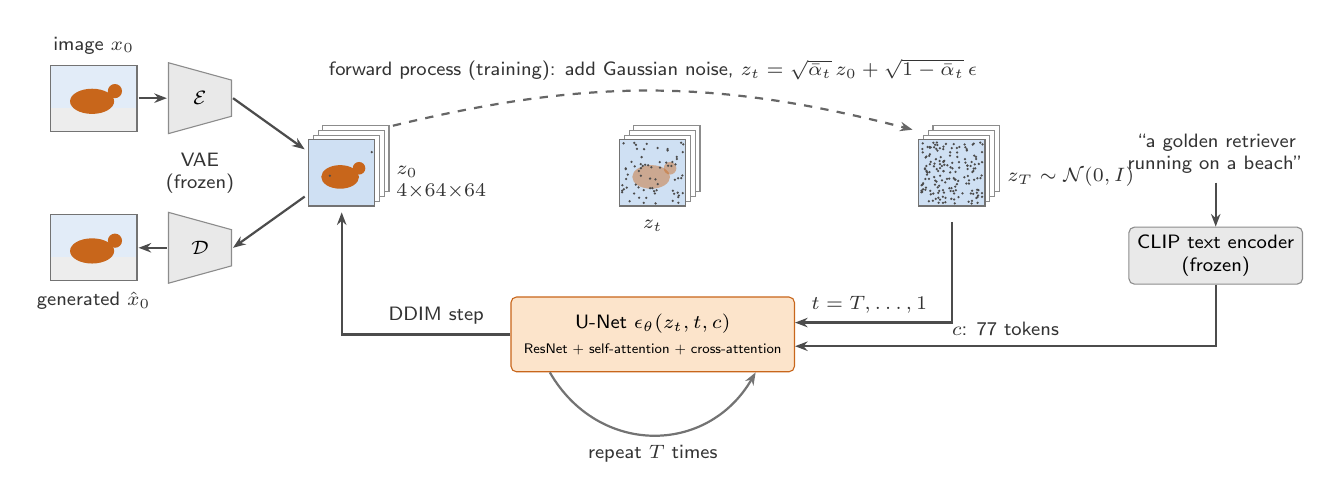
\begin{tikzpicture}

% encoder / decoder (VAE)
\frameimg{0.60}{0.95}
\node[lbl] at (0.60,1.62) {image $x_0$};
\draw[draw=frzD, fill=frzF] (1.55,1.40) -- (2.35,1.18) -- (2.35,0.72) -- (1.55,0.50) -- cycle;
\node at (1.95,0.95) {$\mathcal{E}$};
\draw[flow] (1.17,0.95) -- (1.53,0.95);
\frameimg{0.60}{-0.95}
\node[lbl] at (0.60,-1.62) {generated $\hat{x}_0$};
\draw[draw=frzD, fill=frzF] (2.35,-0.72) -- (1.55,-0.50) -- (1.55,-1.40) -- (2.35,-1.18) -- cycle;
\node at (1.95,-0.95) {$\mathcal{D}$};
\draw[flow] (1.53,-0.95) -- (1.17,-0.95);
\node[lbl, align=center] at (1.95,0) {VAE\\(frozen)};

% latents along the noising trajectory
\latent{3.75}{0}{1}{0}
\latent{7.70}{0}{0.45}{70}
\latent{11.50}{0}{0}{170}
\node[lbl, anchor=west, align=left] at (4.32,-0.12) {$z_0$\\$4{\times}64{\times}64$};
\node[lbl, below=0.48cm] at (7.70,0) {$z_t$};
\node[lbl, anchor=west] at (12.08,-0.05) {$z_T \sim \mathcal{N}(0,I)$};
\draw[flow] (2.37,0.95) -- (3.28,0.30);
\draw[flow] (3.28,-0.30) -- (2.37,-0.95);

% forward process (training): add noise
\draw[->, thick, dashed, black!60] (4.40,0.60) to[bend left=14]
  node[above, font=\sffamily\scriptsize, text=black!80]
  {forward process (training): add Gaussian noise, $z_t=\sqrt{\bar\alpha_t}\,z_0+\sqrt{1-\bar\alpha_t}\,\epsilon$} (11.00,0.55);

% reverse process (sampling): U-Net predicts the noise, one DDIM step at a time
\node[box, minimum width=3.6cm, minimum height=0.95cm] (unet) at (7.70,-2.05)
  {U-Net $\epsilon_\theta(z_t, t, c)$\\[1pt]{\tiny ResNet + self-attention + cross-attention}};
\draw[flow] (11.50,-0.62) -- (11.50,-1.90) -- (unet.east |- 0,-1.90);
\draw[flow] (unet.west) -- (3.75,-2.05) -- (3.75,-0.50);
\node[lbl, above] at (4.95,-2.05) {DDIM step};
\node[lbl, above] at (10.45,-1.90) {$t = T, \dots, 1$};
\draw[->, thick, black!55] ($(unet.south west)+(0.5,0)$) to[out=-60, in=-120, looseness=1.2]
  node[below, lbl] {repeat $T$ times} ($(unet.south east)+(-0.5,0)$);

% text conditioning
\node[lbl, align=center] (prompt) at (14.85,0.25) {``a golden retriever\\running on a beach''};
\node[gbox, minimum width=2.1cm] (clip) at (14.85,-1.05) {CLIP text encoder\\(frozen)};
\draw[flow] (prompt) -- (clip);
\draw[flow] (clip.south) -- (14.85,-2.20) -- node[above, lbl] {$c$: 77 tokens} (unet.east |- 0,-2.20);

\end{tikzpicture}
\end{document}
